\section{Physical problems}
The problems of WTR are not limited to its rear wheels.
There are some more issues that can be resolved in order to improve the stability of WTR.

\subsection{Loose Batteries}
Generally speaking, when something goes wrong electrically, it is because a wire has come loose.
WTR has a different problem, which is illustrated in figure \ref{fig::batteries}.

\begin{figure}[H]
\centering
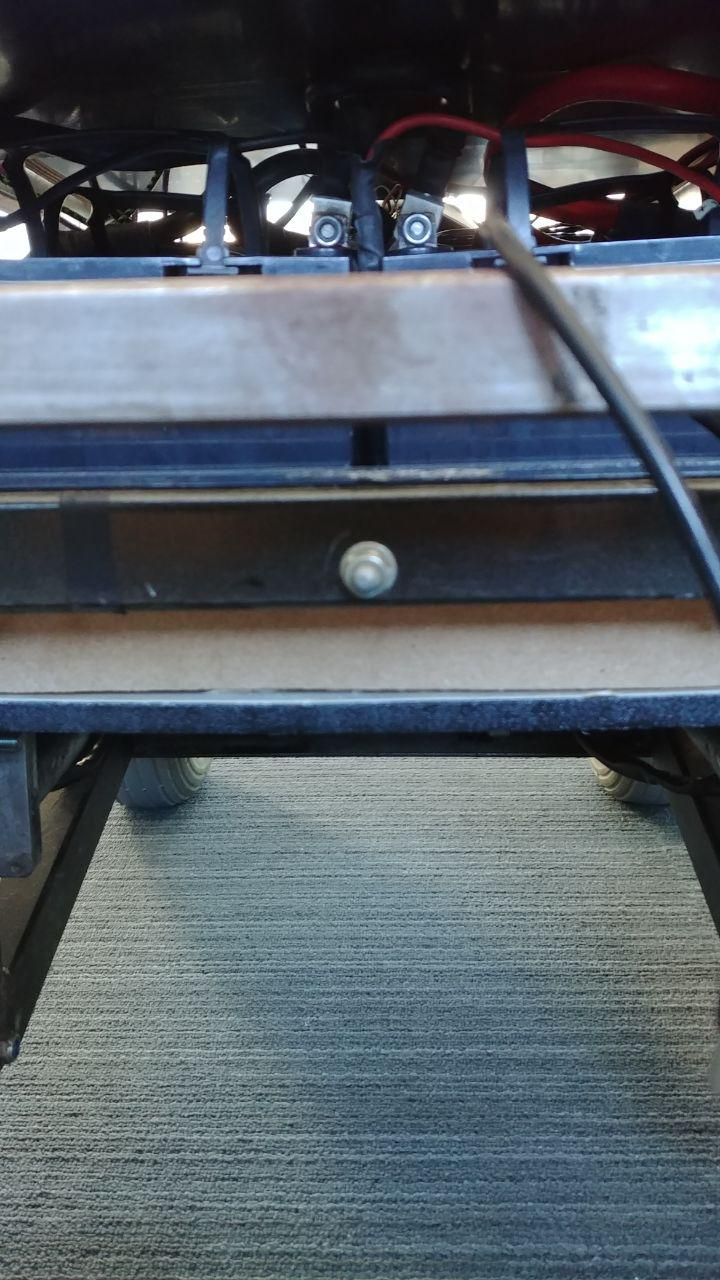
\includegraphics[width=8cm]{batteries.jpg}
\caption{As is slightly visible, the wooden plank is bending}
\label{fig::batteries}
\end{figure}

The wooden plank the batteries are resting on is bending, and the glue/tape which was used to attach that plank is letting go.
While the current situation is not immediately concerning, if WTR were to hit a bump and the force of all the batteries were to hit the plank at once it could snap off of break in two.
That would be a lot of clean-up work for the group, not to mention a lot of work to repair.

Another issue is that the batteries don't have a proper mount, so nothing really keeps them from sliding about.
This means a shifting weight within WTR, which is detrimental to the accuracy of its driving.

These issues are easy enough to resolve.
For the first issue, a metal L-joint around the center of the plank would reinforce the structure so that the bottom falling out would become much less likely.

The second issue can be resolved easily (though not very neatly) by simply wedging some wood or spare non-conductive material between the batteries to keep them from shifting around.
The neater but more time and effort consuming method would be to create a frame that goes over the batteries keeping them in place.
Either solution would suffice, but in order to increase the transferability/quality of the project, the second solution is recommended.

\subsection{Power Converter Box}
Not every component of WTR runs on the voltage levels the car batteries provide.
An Arduino cannot be connected directly to a car battery, so a converter is necessary.
One of the side effects of converting power between different voltages is that a fair bit of heat is produced during the process.
Currently, the converter is located on the rear of WTR, in a plastic lunch box with a fan on it, as seen in figure \ref{fig::converter}

\begin{figure}[H]
\centering
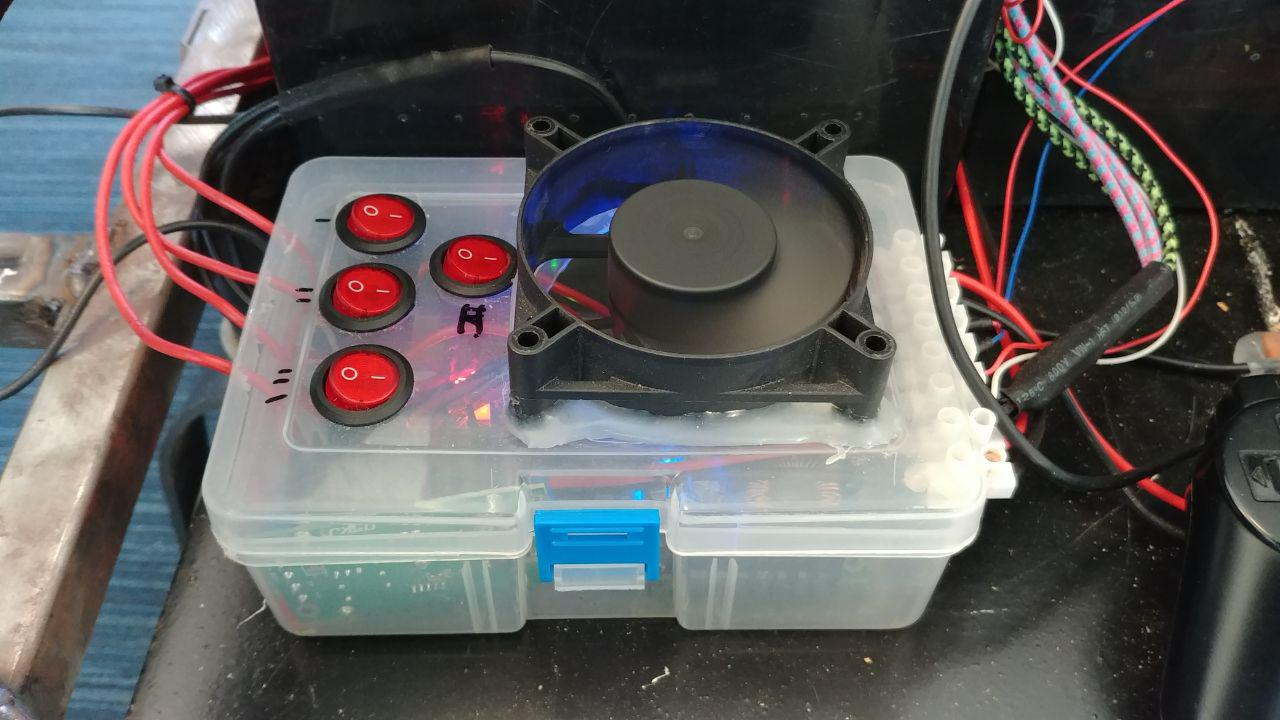
\includegraphics[width=12cm]{converter.jpg}
\caption{Willy's power converter}
\label{fig::converter}
\end{figure}

One of the key issues with this set-up is that while air is being blown into the top of the box, there are no places where that air can escape.
As a result, the air flow in the box is next to non-existent.
While the electrical aspects of the converter are very well executed, this lack of air-flow could mean a reduction in efficiency and useful life-span of the set-up.
By adding a few air-gaps in the side of the box, the air-flow could be improved, leading to a more stable set-up.

It would also be better to have the fan blow in air from the side, so that the hot air can rise to the top more easily, rather than being blows into the box past every other heated object, reducing the efficiency of the cooling further.


\subsection{After Effects of Collisions}
WTR is getting along in its age.
This is the 4th year of its life, and as such it has had to deal with a fair few knocks and scrapes.
One such collision ended up knocking one of the front wheels so that it was stuck at an angle.
As a result, the wheel kept scraping against the frame, and the effects can still be seen in figure \ref{fig::wheelclip}

\begin{figure}[H]
\centering
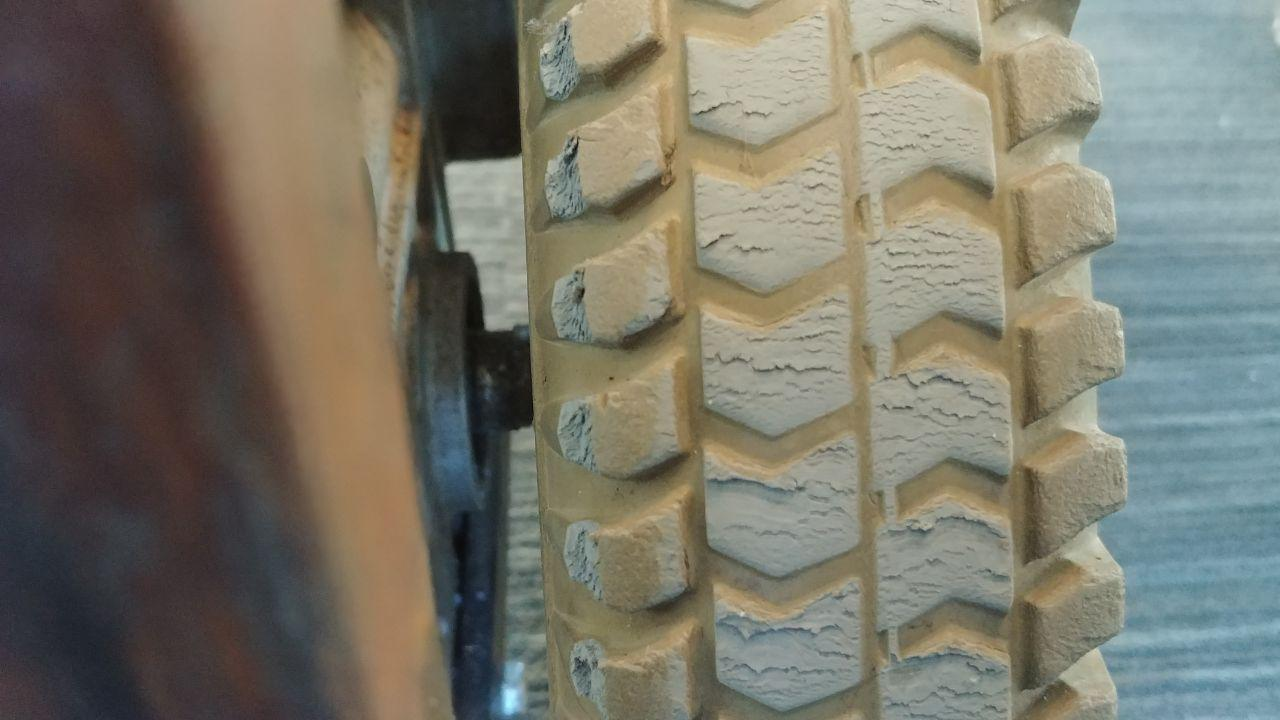
\includegraphics[width=12cm]{clippedwheel.jpg}
\caption{The left side of the wheel shows the damage done by the frame}
\label{fig::wheelclip}
\end{figure}

Another issue which can be seen on figure \ref{fig::wheelclip} is that the tread on the tires is being worn away.
This results in the wheels slipping on the floors of Windesheim, which are mostly smooth, where they are not carpeted.
Since the two wheels are at different levels of wear due to the aforementioned grinding of the tire against the frame, they slip different amounts.
This unfortunately means that the accuracy of any soft-ware based solutions will be lessened.

The effects mentioned above can be counteracted.
When it comes to the clipping issue on the left front tire, it has already been resolved by straightening out the axle and increasing the rigidity of the suspension, causing WTR to stand a little taller and putting a bit of distance between the tire and the frame.

The issue of slipping is not as easy to resolve.
New tires would be a lot of trouble to acquire and replace, and would at best be a stop-gap measure.
Because WTR is so heavy, even without the cover, the tires would get worn down quickly anyway.
The best solution therefore is to either lighten WTR, or attempt to reduce the impact of the slipping.

By adding rotary encoders, the amount of rotations made by both wheels can be tracked, so if one tire keeps slipping, the other can alter its speed to compensate for the turn that would be caused by the different speeds of both sides of WTR.


\subsection{Rear Wheels Issues}
WTR is based of an old electric wheelchair/mobility scooter.
While this does provide a solid base that can carry a good amount of weight, it was never intended to drive autonomously.
Steering is the biggest issue.
When WTR is simply driving in a straight line, (and the wheels are not being interfered with by the frame) it will do so properly.
The engines are mostly synchronised, but since they function independently, as there is no guarantee they move exactly at the same speed.
Issues arise when WTR is attempting to drive in a straight line after a turn.
Because the rear wheels are not motorized and turn on a pivot, they do not straighten themselves in any way, except for being dragged while driving straight.
This issue is illustrated in figure~\ref{fig::mvmnt}.

\begin{figure}[H]

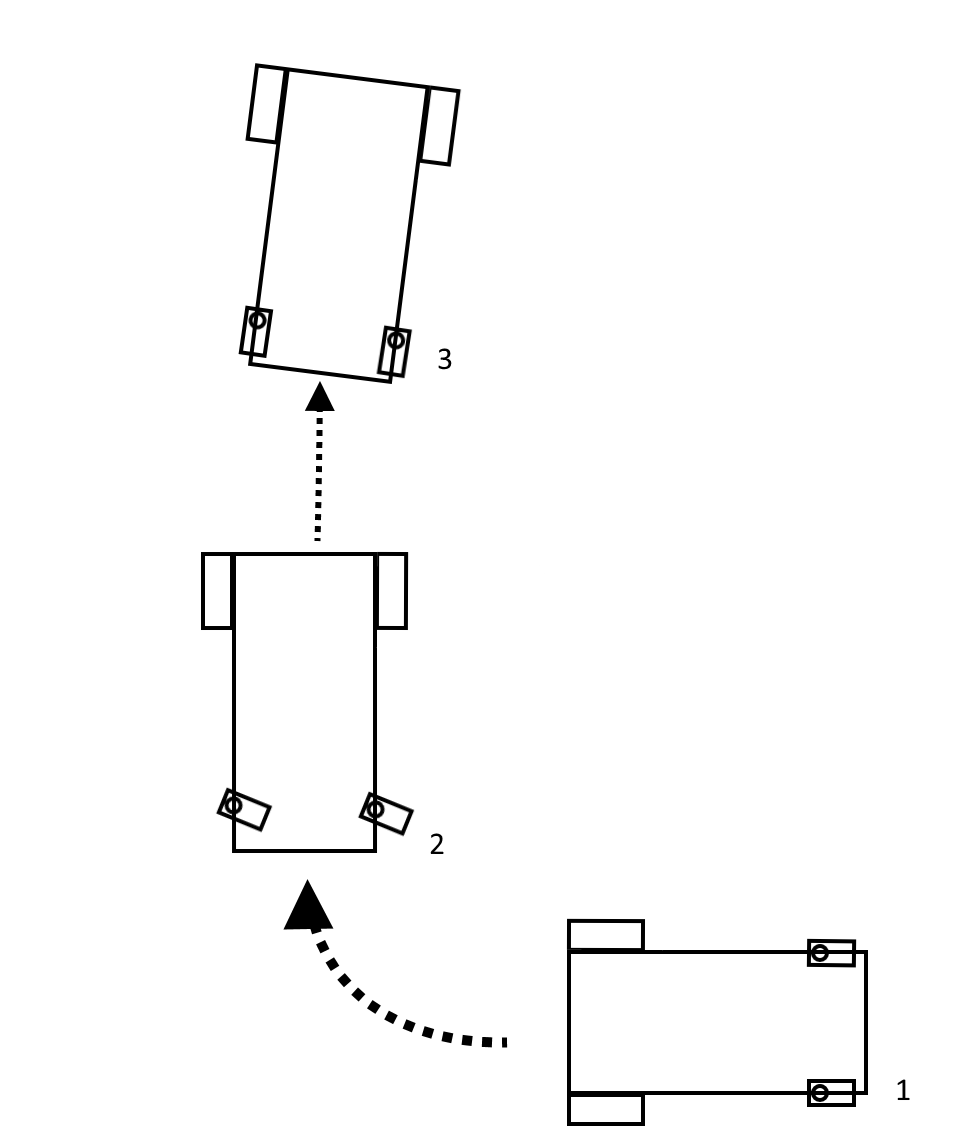
\includegraphics[width=10cm]{movementdiagram.png}
\caption{An approximation of the effect of the rear pivot wheels}
\label{fig::mvmnt}
\end{figure}
As the wheels are not straightened while WTR is facing the desired direction, when driving straight after making a turn WTR gets thrown off course.
This can be compensated for in a few ways.

\begin{labeling}{Single Wheel Bearing}
\item [Tank Controls] By having both the front and rear wheels linked to the motor, steering happens around the center of the wheels, rather than the midpoint between the two frontal wheels. The downside of this is that it would require a compete rework of how WTR is made.
\item [Fixed Rear Wheels] By having the rear wheels have a fixed orientation, the issue of overshooting a turn becomes null, but it creates a new issue of necessitating a larger turning arc, which is counter-productive in a crowded environment.
\item [Single Wheel Bearing] Instead of having a rear wheel, a ball bearing which rolls along the ground and is attached to the frame by a fixture would completely remove all issues of getting the wheels stuck in a direction other than which WTR would need to move, but due to the weight of the frame WTR would have to carry this option is not realistic.
\item [Rotary Encoders] By adding rotary encoders to both the front and rear wheels, it would become possible to track the orientation of the rear wheels and the amount of rotations made by the front wheels. If this is known to WTR, then it can compensate for those issues. When the turn is finished, it can check how the rear wheels are positioned, and if they are not straight, drive in an arc towards its target until the wheels are properly oriented again. 
\item [Front wheel encoders] By not adding rotary encoders to the rear wheels, the cost can be kept down. Since they influence how the front wheels turn through the friction of their pivoting, it is not necessary to know their exact positions.
\end{labeling}

Another issue that the pivot wheels cause is linked with how the ROS move\_ base functions.
This is a generalized system, meant to provide an easy solution to more general applications.
Most of these general solutions are in a style similar to a Roomba \cite{roomba}.
This is used as a general example, since they provide a good visual example.
\begin{figure}[H]
\centering
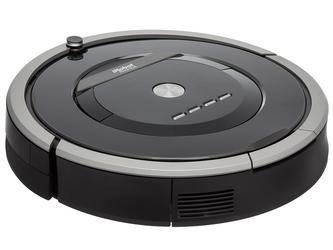
\includegraphics[width=12cm]{roomba.jpg}\
\caption{A Roomba}
\label{fig::Roomba}
\end{figure}

A Roomba can turn around its exact centre, which means that no part ever truly sticks out during a turn.
WTR, unfortunately, has not been built in that manner.

WTR is built in a rectangular shape, first of all.
This means that corners have to be taken into account, necessitating a wider turn arc, or it would risk hitting objects.
Another issue that complicated matters is that it does not turn around its exact center.
Instead, it turns on an axis located between the two front wheels, which means the rear side sticks out quite far when turning.
The ROS move\_ base does not compensate for this, and RVIZ, the path-finding tool used, does not allow for custom polygons that dictate the shape of the robot.
This means that its footprint in the calculations has to consider the largest WTR can be in any given direction to be the amount WTR extends from the turning point to the rear.

The knock-on effect of this is that WTR considers itself much wider than it actually is during any given calculation.
While this does mean that it will keep more distance from potential hazards, it also means that it will avoid a narrower area it could actually pass through, because it could not possibly turn there.

There are a few solutions to this issue.
\begin{labeling}{Reworking the wheels}
\item [Accepting it] While not desirable and lowering the efficiency of WTR movement patterns, simply accepting that this is the case would save a lot of time, and prevent a rework of the current system.
\item [Changing Software] There are solutions for pathfinding which allow for custom polygons that do not require a central turning point to be in the exact centre of the robot, but applying this solution would take a lot of time and a major rework of existing solutions.
\item [Reworking the wheels] If WTR were to be reworked physically, the rear wheels could be replaced by a set of wheels linked to the engines as well. That way, it could steer like a tank and pivot around the exact centre of the robot. Unfortunately, this would be a very time consuming process.
\end{labeling}

As the latter two solutions would require extensive reworking of either the software or the hardware, it seems that simply accepting that WTR is not going to be extremely efficient is the only course of action.

\newpage